\chapter{Action--sound couplings}\label{chapter:couplings}

`Toot Whistle Plunk and Boom.' That is how the history of Western musical instruments was introduced in Disney's 1953 cartoon of the same name. The four words are onomatopoeia for the sounds of brass, woodwinds, strings, and percussion instruments, respectively. I often show the cartoon when lecturing about instruments. It is funny, yet remarkably illustrative of what I call \emph{action--sound couplings}. I call these couplings because there is always a sonic result when you act on a physical object, as sketched in Figure~\ref{fig:instrument2}. If you interact lightly, the sound may only barely be audible. But it will be there if you listen carefully, and certainly if you attach a contact microphone to the object in question.

\begin{figure}[tp]
  \centerline{
      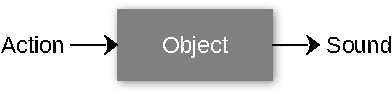
\includegraphics[width=.5\columnwidth]{figures/36-object-sound-crop.pdf}
      \caption{Acting on a physical object will lead to sound production.}
            \label{fig:instrument2}}
\end{figure}


\section{Sound-source perception}

An action--sound coupling can be described in terms of the acoustic properties of the objects involved and the (bio)mechanics of the sound-producing action. Given the same physical objects and actions, the resultant sound will always be the same. This is also reflected in the way we perceive the interaction. Our life-long experience with various objects makes us able to predict the sonic result of many actions on those objects. This means that we can predict the resulting sound of an interaction even before it is heard.

We can verify our mental capacity for predicting the outcome of an action--sound coupling in a thought experiment. Think back at the exammple of the glass falling towards the floor. While still in flight, you will imagine both the visual and auditory results of the glass breaking to pieces when it hits the floor. Knowing that the sound will be unpleasant, you may even try to cover your ears to protect your hearing. This example demonstrates that we immediately understand the sonic properties of the objects involved, the actions on those objects, and the resultant sounds. This knowledge can be used to estimate both the timbral qualities and loudness of the sound to emerge based solely on the glass' visual information and its trajectory in the fall. Such tacit \emph{psychomechanical} knowledge guides us in also telling the approximate size of the glass, the surface it hit, the distance it fell, whether it was dropped or thrown, and so on \citep{mcadams_psychomechanics_2000}.

Let us turn the thought experiment around and start by imagining that you only \emph{hear} the sound of a glass breaking to pieces. Even though only the audition is activated, you will be able to tell much about the objects and actions involved. Researchers in sound-source perception have uncovered our remarkable ability to perceive the qualities of the materials and actions associated with sounds only from listening \citep{gaver_how_1993,gaver_what_1993}.
This ability to identify the properties of objects based solely on sound seems to be surprisingly reliable and accurate. It is robust during attentive listening and in the everyday perception of impact sounds and sources \citep{rocchesso_sounding_2003}. This is logical from an ecological perspective, considering that characterizing and identifying sounds is essential in the interaction with objects in the environment.
This means that we can recognize qualities of specific types of sounds, such as bouncing and breaking bottles \citep{warren_auditory_1984}, clapping hands \citep{repp_sound_1987}, mallets striking pans \citep{freed_auditory_1990}, the amount of liquid in a cylinder \citep{cabe_human_2000}, the direction of a sound source in three-dimensional space \citep{neuhoff_perceiving_2001}, the length and hollowness of objects \citep{carello_perception_1998,lutfi_auditory_2001},
their shape \citep{kunkler-peck_hearing_2000}, the material categories of struck objects of variable sizes \citep{giordano_material_2006}, and so on. I find these and similar studies fascinating because they attest to the richness of our auditory system. They also support my main argument that action--sound couplings are essential in our interactions in the world.


\section{Excitation and resonance}

The physics of action--sound couplings are generally well understood. So are the basic psychoacoustic principles. Then there are more open questions about how they are perceived by our (embodied) cognitive system. \citet{godoy_imagined_2001} has suggested that our cognition of sound-producing actions may be based on `images' of sonic features. Such mental images should be understood as `quasi-perceptual' experiences that resemble real perceptual experiences but with the absence of external stimuli \citep{thomas_mental_2007}. Even though the word `imagery' may draw attention towards the visual, all modalities are included when `mental imagery' is used. This includes both `seeing in the mind's eye' and `hearing in the head.' Therefore, the term `musical imagery' can be understood as the mental capacity for imagining musical sound in the absence of a directly audible sound source. Given the close connections between action and sound, such a `hearing' of sound in your mind would also mean that you `see' the accompanying sound-producing action.

In his elaboration on the mental imagery related to musical sound, \citet{godoy_imagined_2001} further suggests that such imagery can be divided into \emph{motor images} and \emph{material images}. Here the motor images are mental representations of the excitation of an object. The material images represent the resonances of the sounding objects, which indicates the properties of the objects. I would argue that we also hear one extra layer of resonance: the \emph{environment}. If you imagine a drum stroke, for example, you will be able to hear the drum and its properties (size, shape, materials) and the object that hit the drum and its properties (hand, stick, mallet). You will also most likely hear the room within which the sound appeared and its properties (small/large, dry/wet, and so on). These different layers are summarized in Figure~\ref{fig:excitation-resonance}. The sounds of the environment are studied within room acoustics--- a different field from instrument acoustics---and have often been neglected in many discussions about instruments. While this makes sense in many situations, I have found that it is necessary to take this layer into account to understand the differences between acoustic and electro-acoustic instruments.

\begin{figure}[tp]
  \centerline{
      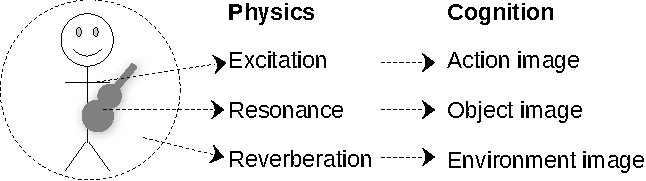
\includegraphics[width=.8\columnwidth]{figures/37-physics-cognition-crop.pdf}
      \caption{The mental imagery of sounds can be broken down into three components: images of the actions, the object(s), and the environment.}
      \label{fig:excitation-resonance}
      }
\end{figure}


In a further development on his thinking on musical imagery, \citet{godoy_gestural-sonorous_2006} suggests that our cognition of sound objects is based on mentally `tracing' features of the sound while listening, or even when only imagining, music. This was the idea behind the sound-tracing studies described in Chapter~\ref{sec:accompanying}. These studies showed no one-to-one relationship between the physical properties of the involved actions and their imagined sonic counterparts. We do not, for example, see a guitar when hearing a guitar-like sound, but we get an embodied sensation of strings and a vibrating body. In my extended model, we also get an embodied feeling of the physical or virtual space where the vibrating body is located.


\section{The sound object}

The model of musical imagery put forwards by \citet{godoy_imagined_2001} builds on the thinking of \citet{schaeffer_solfege_1967} on \emph{reduced} listening. This is a particular type of listening that is focused on the sound `itself.' At the core of Schaeffer's theory is the identification of \emph{sound objects}, fragments of sound perceived as one coherent unit.
Sound objects can last up to a few seconds but are often shorter. The main point is that they are perceived holistically as an `object' with a shape. It may seem paradoxical that I use the concept of a sound object in discussions of its sound-producing action. After all, Schaeffer explicitly wanted to listen to sounds without considering the sound source. The aim was to use sound material in his compositional practice. Schaeffer did this by cutting and splicing sound recordings so that the original sound source was unidentifiable. He also discovered that much of the source information was lost when cutting off the beginning of the sound, the attack part. This made it possible to listen to the timbral qualities of the sound and not get stuck with mental imagery related to the objects and actions involved in sound production.

Several composers and music researchers have extended Schaeffer's thinking over the years. \citet{smalley_spectromorphology_1997} has developed his \emph{spectromorphology}, which refers to the interaction between sound spectra (the \emph{spectro-}) and how they are shaped through time (the \emph{-morphology}). \citet{thoresen_Emergent_2015} have developed a complete visual language for spectromorphological analysis. Common to their---and Schaeffer's---thinking is that the sound should be considered without reference to its source. \citet{smalley_spectromorphology_1997} refers to this as getting away from `technological listening,' that is, listening for the techniques of sound production rather than the sound itself. In acousmatic music, the loudspeakers are the physical sources of the audible sound. The sound's identity, however, is not visible. Still, there may be cases in which the listener try to (willingly or unwillingly) locate the source of a sound, what \citet[p.110]{smalley_spectromorphology_1997} refers to as `source bonding':

\begin{quotation}
   [\ldots] the \emph{natural} tendency to relate sounds to supposed sources and causes, and to relate sounds to each other because they appear to have shared or associated origins.
\end{quotation}

\citet{godoy_gestural-sonorous_2006} argues that despite the seemingly `disembodied' nature of Schaeffer's thinking, there is no conflict between the principles of reduced listening and those of embodied cognition. Instead, there are several similarities between studying sound objects and their sound-producing actions from a phenomenological perspective. This is the case also for my thinking about the cognition of action--sound couplings. When we hear a guitar-like sound, we get a sensation of an impulsive-like attack. Such a pluck on a guitar will result in quite different imagery than when hearing the bowing on a cello, even though both are string instruments with similarly shaped bodies. It is also interesting to consider the difference between hearing plucking versus bowing on a string instrument like the cello. The sounds would be perceived differently, but the sound source (the cello) would probably be heard. This is an example of how excitation and resonance play together in the cognition of sound objects. It is important to remember that this model is bi-directional. Hearing a sound object will evoke the mental image of a sound-producing action. Similarly, seeing a sound-producing action will evoke a mental image of the corresponding sound object.

Developing this thinking one step further, \citet{launay_musical_2015} argues that listening to music is an inherently social experience, even when it happens alone. He proposes a model in which the detection of human agency is at the core of the musical experience. This is based on learning relationships between sound, action, and agency.
\citet{launay_rapid_2016} followed up with an empirical study in which non-musicians were asked to quickly learn new associations between sounds and observed actions without performing those actions themselves. The researchers measured the motor evoked potentials (MEPs) in the participants’ right hands and used single transcranial magnetic stimulation (TMS) pulses to trigger motor activity. The results showed that observers could quickly learn to associate sound with action. This indicates that it is not necessary to have played an instrument to experience some motor resonance when hearing that instrument.

Most of the literature that I build my action--sound theory on have explicitly tried to get away from understanding the sources of sounds, whether these sources are instruments or other types of sound-making objects. However, as mentioned above, there is not necessarily a conflict between understanding (and appreciating) the qualities of sounds while at the same time reflecting on how they are produced. In fact, knowing more about the perception of acoustic sounds may help create better and more interesting electro-acoustic sounds. Therefore, let us move from the general thinking about action--sound couplings to some more music-specific examples.


\section{Action--sound couplings in instruments}

As mentioned in Chapter~\ref{sec:voice}, \citet{paine_interaction_2015} has proposed the term \emph{techno-somatic dimension} to describe what is happening between the physical instrument and the human body. He argues that the techno-somatic dimension is the \emph{somatic gestalt} formed between the physical instrument and the human body's intentional actions. This somatic gestalt represents the instrument's cumulative experience, enacted through technique and experienced through somatosensory and listening phenomena. This relates to my thinking about the action--sound palette of an instrument (or any other sound-producing object).

Paine further argues that many new designers of new instruments/interfaces have forgotten the techno-somatic dimension. The most significant problem with general-purpose interfaces, he argues, is that they do not offer an idiomatic playing style. Many standard acoustic instruments have a clearly defined playing technique, which helps develop performance skills, pieces, and educational material. To make successful new instruments, Paine suggests putting the techno-somatic dimension on top of the design priority list. He also argues that building on existing instrument designs makes it possible to draw on the transferable skills of `neighboring' instruments. I partly agree with this but will later reflect on some challenges assuming that skills are transferable between devices.

The generic, one-directional action--object--sound chain presented in Figure~\ref{fig:instrument2} does not reveal the \emph{inter}action going on in musical performance. Typically, there is a continuous loop of actions exerted on the instrument by the performer and \emph{re}actions from the instrument to the performer, as sketched in Figure~\ref{fig:instrument3}. The actions excite the instrument, which leads to vibrations in the instrument body. These vibrations lead to audible sound, and they also lead to haptic feedback to the performer.

\begin{figure}[tp]
  \centerline{
      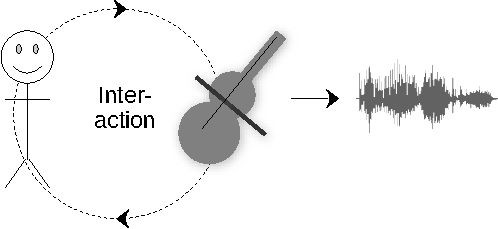
\includegraphics[width=.6\columnwidth]{figures/38-interaction-crop.pdf}
      \caption{An instrument can be seen as a mediator between action and sound, including a constant feedback loop between instrument and performer.}
            \label{fig:instrument3}
}
\end{figure}

Most instruments are constructed from multiple parts, and many may also be played with one or more tools. For example, the two most essential parts of a violin-like instrument are the strings (the \emph{vibrator}) and the instrument body (the \emph{resonator}). To produce sound, we also need a bow (the \emph{excitator}), as sketched in Figure~\ref{fig:instrument4}. Many percussion instruments are tool-based, while brass and wind instruments are not. In the latter, the excitation happens at the meeting point between lips and mouthpiece. Still, all of these instruments rely on an instrument body that acts as a resonator.

\begin{figure}[tp]
  \centerline{
      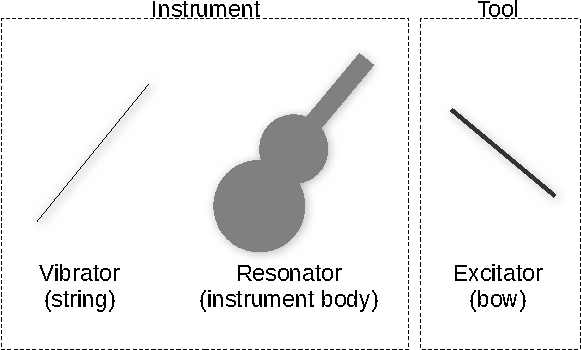
\includegraphics[width=.7\columnwidth]{figures/39-tools-crop.pdf}
      \caption{A string instrument makes sound with a vibrator, an excitator, and a resonator.}
            \label{fig:instrument4}
}
\end{figure}

I will not go into further details of instrument acoustics here, but interested readers can check out the excellent overview in \citet{rossing_science_2002}. Here we will keep the discussion at a system level, from which it can be argued that the result of an interaction with an instrument ultimately boils down to the physical interaction between the objects involved, which again will be based on the following parameters:

\begin{itemize}
\item the instrument body and its vibrating parts
\item the tool(s) used to play the instrument
\item the sound-producing action
\item the environment within which the interaction happens
\end{itemize}

As mentioned in the discussion about mental imagery, the environment is often forgotten in conversations about instruments. Even though most musicians have preferences for particular environments, most would probably think about their instrument as moving from space to space. However, as we shall see later, there are also cases in which the environment is crucial for how an instrument is performed and perceived. So I am in favor of including the room that the instrument is played within as part of a general instrument model (Figure~\ref{fig:instrument5}).

\begin{figure}[tp]
  \centerline{
      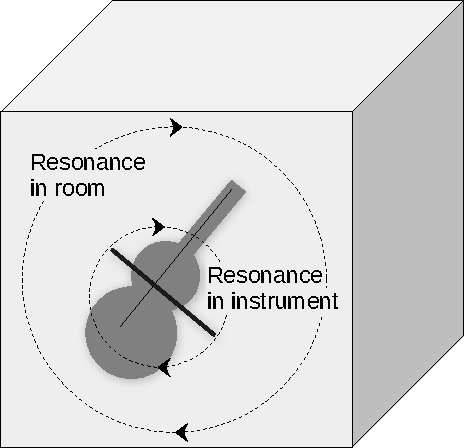
\includegraphics[width=.5\columnwidth]{figures/40-room-crop.pdf}
      \caption{A sketch of the two layers of resonance, one in the instrument body and one in the room.}
            \label{fig:instrument5}
}
\end{figure}


\section{Action--sound palette}\label{sec:palette}

As discussed in Chapter~\ref{sec:affordance}, an object can have multiple affordances, that is, invite different types of usage. It may also have numerous sonic affordances. These sonic affordances are related to the size, shape, materials used, and construction of the sound-producing objects involved in an interaction. The sonic affordances help set up an action--sound palette of possible couplings between actions and sounds. So an action--sound palette can be seen as our combined knowledge of the properties of sounding objects and possible sound-producing actions.

Action--sound palettes are probably deeply rooted in our cognitive system and is something we activate continuously in our interactions in the world. This helps us avoid making unnecessary loud sounds when we move around. Other times, we may want to make sound to let others know that we are coming. The same system is activated in musical practice. For example, think about how you can make music with a wine glass. You can use it as a percussion instrument by tapping on the side with your finger. Tapping with the fingertip will result in a different sound than using the nail. Both would be examples of impulsive sound-producing actions, albeit with different sonic results. You could also wet your finger and move it in a circle on the top of the glass to produce sound. Furthermore, the pitch of the sound could be modified by pouring water into the glass. These possible sonic affordances (and more) would together constitute our understanding of the action--sound palette of the glass.

As we shall see later, the idea of a constrained action--sound palette does not work equally well for action--sound mappings in electro-acoustic instruments. In theory, any combination of action and sound can be designed and created digitally. This makes it difficult to set up a similar set of expectations for an action--sound mapping than you would for an action--sound coupling. When you touch the key on a keyboard-based synthesizer, it is impossible to know what type of sound you will get.


\section{Action--sound separation}\label{sec:separation}

The concept of an action--sound palette helps define the possible sonic outcomes of an interaction. As we move towards discussions of musicking machines, it may also be relevant to have a conceptual apparatus for talking about the body's involvement in the sound production.
\citet{keislar_historical_2009} uses the term \emph{disjunction} to explain the increasing disconnection between action and sound throughout the development of instruments. To create a more fine-grained terminology of such disjunctions, I will introduce the term \emph{action--sound separation} to describe how close (or far) the body is related to the sound-producing object. This is inspired by the Hungarian composer Bela Bartók's organization of instruments according to their closeness to the human body. In a 1937 essay on mechanical instruments, \citet[p.289--290]{bartok_mechanical_1976} suggested a continuum from the human voice, followed by wind instruments, bowed string instruments, plucked string instruments, pianos, organs, barrel organs, player pianos, gramophones, and, finally, the radio.

Inspired by Bartók's continuum, \citet{thelle_making_2010} suggested five levels of action--sound separation in instruments: incorporated, direct, mechanical, analog, electronic, and digital.
\citet{enders_idiophone_2017} has identified ten developmental stages from the human voice to virtual musical instruments: instrumentalization, mechanization, automatization, electronification, modularization, digitalization, virtualization, globalization, informatization/artificial intelligence, and hybridization.

There are compelling arguments for thinking about a continuum from the most embodied acoustic instruments to the purely digital ones. However, based on my techno-cognitive reasoning, I believe there are even better arguments for thinking about acoustic and electro-acoustic instruments as two separate categories. After all, acoustic instruments are based on action--sound couplings governed by the laws of physics, while electro-acoustic instruments are based on designed action--sound mappings. In my current model, I have, therefore, decided to keep them separate.

We will start by considering the action--sound separation of acoustic instruments and return to electro-acoustic instruments in Chapter~\ref{chapter:mappings}. I propose the following elements of a continuum describing the action--sound couplings in acoustic instruments:

\begin{itemize}
  \item Embodied: Sound is produced with(in) the human body, such as the voice or clapping.
  \item Tactile: The human body is in direct contact with resonating objects, such as in the guitar or flute.
  \item Tool: There is a simple tool between the body and the instrument, such as in the sticks used in percussion or bowing in string instruments.
  \item Mechanical: Two or more mechanical elements (levers, pulleys, and so on) are involved in the excitation, such as in the piano.
  \item Automatic: There is no physical contact between the body and instrument during excitation, such as in a self-playing piano or music box.
  \item Conceptual: There is no physical instrument to interact with; the instrument and its sound-production are only happening within your (embodied) mind.
\end{itemize}

The idea of the continuum is to reflect on how the interaction goes from being wholly embodied to completely disembodied, as sketched in Figure~\ref{fig:instrument7}.
The traditional organological definitions presented in Chapter~\ref{sect:organology} are primarily object-based. However, one could argue that the Hornbostel Sachs system also contains information about how the objects can be played. My model, on the other hand, is entirely (inter)action-based. While this also has its limitations, one immediate benefit is that the voice can be easily included in the model. This makes sense from a performance and perception perspective. After all, the voice is probably the most commonly used musical instrument.

\begin{figure}[tbp]
      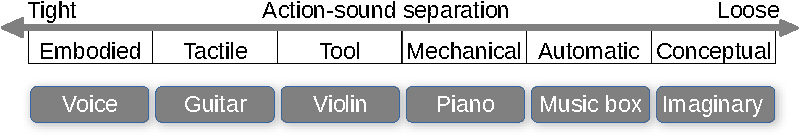
\includegraphics[width=\columnwidth]{figures/41-separation-crop.pdf}
      \caption{A sketch of how we may think of a continuum with an increased level of action--sound separation.}
            \label{fig:instrument7}
\end{figure}

The action--sound separation presented here should be seen only as an indication of different functions. In practice, however, there are often many possible combinations. For example, string players may be in direct contact with their instrument using the left hand while playing it with a tool (a pick or a bow) with the right hand. We may also find apparent differences between excitation and modification actions regarding the level of embodiment. Therefore, it may be relevant to develop a two-dimensional continuum, to include both excitation and modification actions (Figure~\ref{fig:instrument8}).
In the following, I will go through each of the main categories and consider how different instruments can be placed within the system.

\begin{figure}[tbp]
      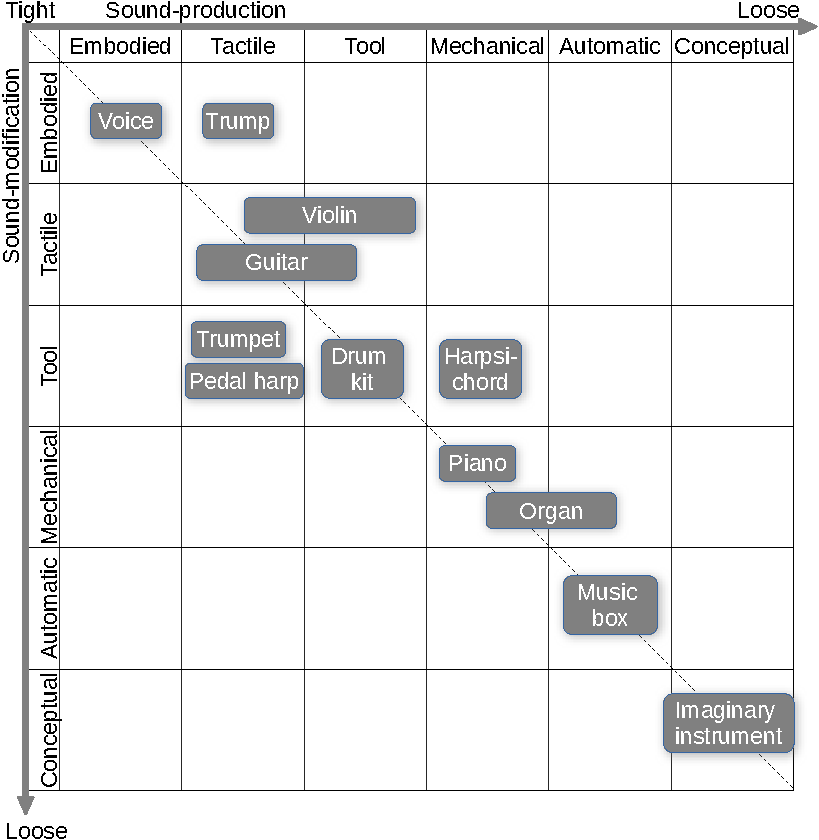
\includegraphics[width=\columnwidth]{figures/42-separation2-crop.pdf}
      \caption{Action--sound separation in two dimensions: excitation and modification of sound, from tight to loose in both dimensions.}
            \label{fig:instrument8}
\end{figure}


\subsection{Embodied instruments}

As should be clear by now, I favor thinking about the body itself as an instrument. The body can create lots of sounds on its own, many of which are used in musical contexts. The voice is an obvious example of an embodied instrument. It may be argued that the body was not made for musical purposes. However, it has also been suggested that human musical activity has its origins in vocalization \citep{mithen_singing_2006}. The body can also produce many non-vocal sounds, both intentional and unintentional. Hand clapping is an example of intentional non-vocal body sound. There are numerous unintentional body sounds, of which several have been explored in experimental performances. I still vividly remember a performance in the Yerba Buena Gardens in San Francisco of the piece \emph{The Sound of Naked Men} by Miya Masaoka. Here the sounds of the bodies were amplified using stethoscopes placed on the bodies of the performers. The instrument in this performance was more of a hybrid nature, with amplification of the acoustic sound sounds from the performers' bodies. The same is the case in Marco Donnarumma's works exploring muscle sounds in music performance \citep{donnarumma_configuring_2016}. He also works electro-acoustically, relying on heavy signal processing of the original acoustic sound signals. Still, the original sound source is the acoustic sound of the body. We will return to further discussions of such hybrid instruments in Chapter~\ref{chap:hybrid}.


\subsection{Tactile instruments}

The tactile category includes instruments in which the performer's body directly touches the sound-producing element. A hand drum is an instrument where the performer both excites and modifies the sound directly with the hand. In a recorder, the performer excites the instrument by blowing directly into the mouthpiece and where the fingers are in direct contact with the vibrating sound when closing the holes. When played with the fingers, the guitar is another example of a tactile instrument. On the other hand, if one plays on the strings with a plectrum, it would be classified as tool-based sound production. However, the left hand would still be in direct contact with the guitar. So a plectrum-based guitar performance would be classified as tool-based on the sound-production axis and tactile on the sound-modification axis.

There are several other borderline cases within the tactile category, and which may be placed outside the diagonal in the system sketched in Figure~\ref{fig:instrument8}. As discussed earlier, the trump (Figure~\ref{fig:munnharpe}) is an instrument in which the sound production is tactile since the performer is in direct contact with the instrument's vibrating element. However, sound modification is primarily happening in the performer's mouth and could be classified as embodied. It could be argued that the same is true for woodwind instruments, such as a saxophone. Here, the mouth's cavity is an integral part of both the creation and modification of sound. The creation of saxophone sound happens in the reed and is amplified in the instrument's body. The difference between a saxophone and a trump is that the trump does not have any `amplifier' built-in. Instead, it relies on the creation of resonance inside the mouth. So I would still argue that there is a difference between a trump and various wind instruments with built-in resonators. This also holds for brass instruments. Here the performer is producing audible sound with the lips before it enters the mouthpiece. So the excitation of a brass instrument could be considered partly embodied. The modification, too, perhaps, considering that it is possible to shape the sound with the lips. Changing tones can also be done by adjusting the pressure of the lips.


\subsection{Tool-based instruments}

The next level of separation between action and sound is when there is some kind of tool between the performer and the sound-producing element. A simple example is that of a drum played with sticks. Here both the excitation and modification are separate from the performer's direct touch (and feel).  If we compare this to the hand-drum included as a tactile instrument, the performance style defines how we characterize the instrument. If the performer plays the drum with the hands, it is classified as a tactile instrument. When playing with sticks, it is tool-based. While this may seem strange at first, it makes more sense when thinking about how the instrument is perceived. Think about the difference between the sound of a drum played with hands and with sticks? The tactile and haptic experiences are entirely different for the performer, which will also influence the perceiver. Even if one were to only listen to (or only see) a performance of hand-played versus stick-played drum music, one would immediately hear the difference and set up different mental imagery.


\subsection{Mechanical instruments}\label{sec:mechanical}

Instruments in this category rely not only on a single tool but some kind of mechanical system. The piano can be thought of as the prototypical mechanical instrument with its complex hammer system. To simplify what happens, we can say that the performer hits the key, which hits the hammer, which hits the string. As such, the performer only has indirect control of the final sounding result. It is interesting to read the reflection of \citet[p.289]{bartok_mechanical_1976} about the piano as a percussion instrument:

\begin{quote}
It is apparent that we should define mechanical music---in the wider sense of the term---as a music in whose creation not only the human body but also some kind of machine is involved. We are accustomed to define the machine, in the everyday sense of the term, as a rather complex construction which serves the purpose of energy transfer. But in the course of our high school studies in physics we have met with simple machines too, such as levers and pulleys. Therefore, if a lever is a machine, then any music is also mechanized music if its origin derives from the use of levers in conjunction with the human body. Having made that statement, of which instrument are we reminded? Undoubtedly the piano, since man's finger on that instrument makes use of a series of levers for energy transfer.
\end{quote}

The piano is but one of many different types of keyboard instruments. The clavichord is one of the `simplest' keyboard instruments, with a more straightforward mechanical construction than its siblings: the harpsichord, virginal, and spinet. In Figure~\ref{fig:instrument8}, the clavichord is categorized as mechanical on the excitation axis and as tool-based on the modification axis. This is debatable but is based on the fact that it is possible to continuously control the string on the clavichord after it has been excited. This makes it possible to modify the sound as if one were playing it directly with a tool.

The organ is another borderline case of mechanical instruments. A typical pump organ would be categorized as having both mechanical excitation and modification. However, how should one think of the stops and the ability to play on multiple pipes simultaneously? Here the organ kick-starts the era of modern-day synthesizers in that it can produce more complex tones through advanced routing of the sound. As such, it may be closer to an automatic than mechanical instrument. When it comes to excitation, a church organ needs a massive airflow to create sound. This airflow has been produced in several ways throughout the centuries \citep{bush_organ_2004}. There are reports of organs based on the kinetic energy of falling water as early as in the Roman era, and some of the pump organs can store air in large bags. Then the instrument could almost `play itself' as an automatic instrument. However, most pre-electric organs rely on manual pumping. Some are based on foot pedaling by the same person playing the keys. In the large church organs, there often had to be multiple people involved in creating the airflow. This is an early example of a multi-performer instrument, according to my definition. Most likely, only the person sitting at the keys would be called a musician, but I would argue that the people pumping air should get credit for their musicianship.


\subsection{Automatic instruments}\label{sec:automatic}

The automatic category includes instruments that can play without the direct energy transfer of a human performer in one way or another. This includes everything from small music boxes to self-playing pianos. There are also examples of traditional instruments equipped with self-playing mechanisms operated by a human performer, such as the pianola. I will not go into detail about all the different types of automatic instruments here, but interested readers can see \citet{bowers_encyclopedia_1972} for an extensive overview.

Music boxes, such as the ones in Figure~\ref{fig:music-box}, may be seen as  forerunners of today's musical reproduction systems. While they differ widely in construction, such music boxes have in common that they are music-makers; they embed the musical score. In some cases, the scores are stored as holes on paper roles. Other times they are engraved into holes on metal plates or added as spikes on metal cylinders. These can then be played back by the instrument, often with a high level of temporal precision and with dynamic articulation. Some music boxes can be controlled directly by a human performer, while others are self-playing. This is achieved through the preservation of energy in the instrument. Some self-playing instruments use airbags, but many rely on spring systems. These are typically wound up with a crank, after which they can play on their own.

\begin{figure}[tbp]
     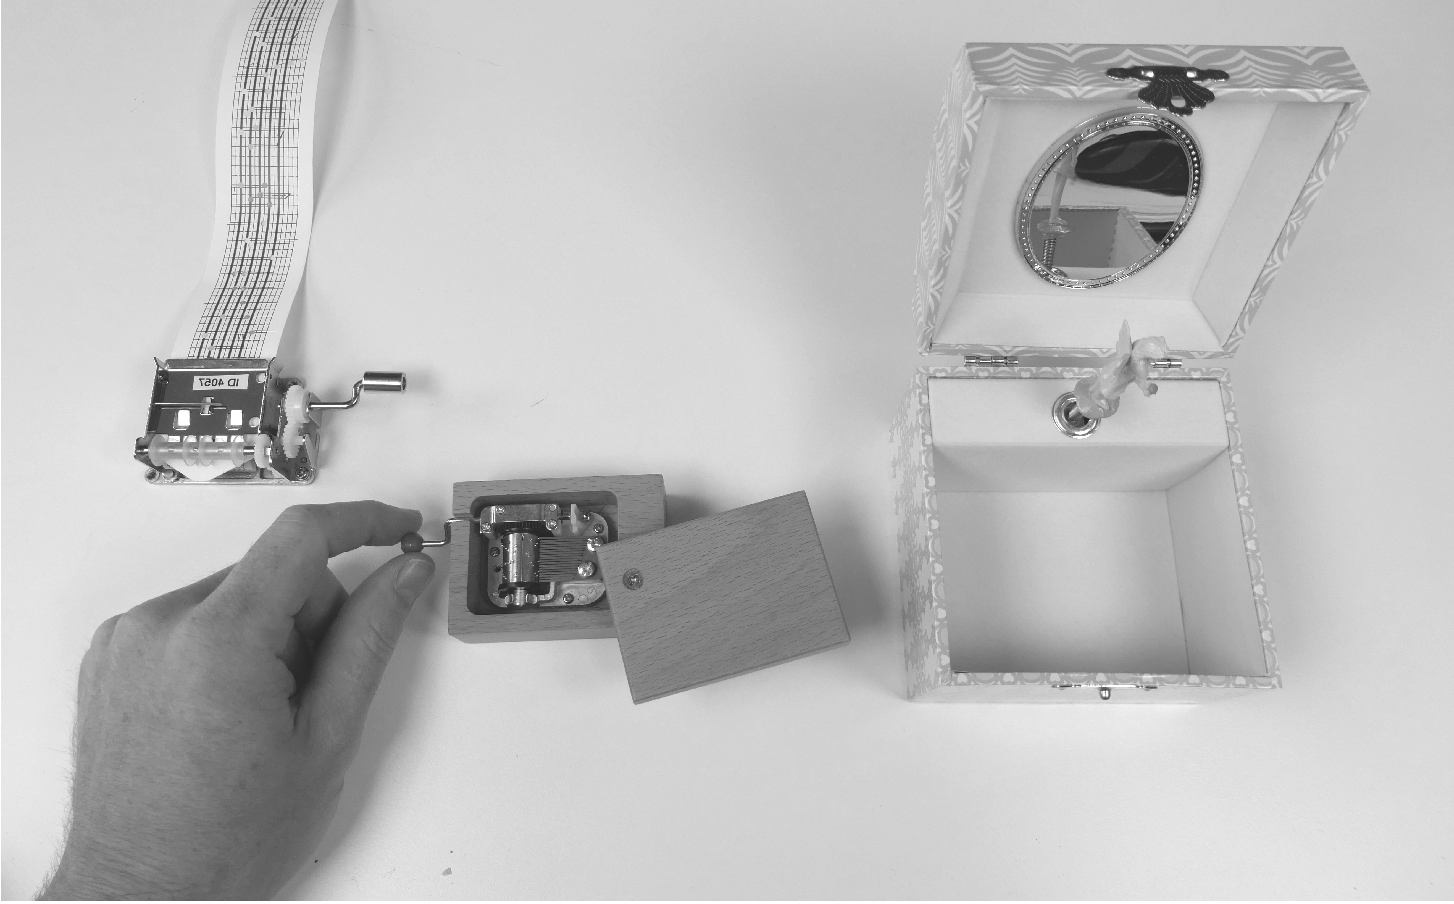
\includegraphics[width=\columnwidth]{figures/43-music-box-crop.pdf}
     \caption{Examples of a regular music box with a small resonance chamber (middle), a customizable music box with interchangeable paper scores (left), a self-playing music box with a crank on the back (right).}
     \label{fig:music-box}
\end{figure}

Some question whether automatic instruments should be considered `real' instruments. Yes, is my answer. To reflect a little more on the question, let us consider another atomatic instrument: the pianola. Many pianolas have a standard keyboard and can be played as a mechanical instrument. The only difference from an ordinary piano is that they can also play independently. In some pianolas, the energy input is done in real-time using a crank or foot pedals. In that case, the sound production relies on a human performing in in-time and real-time. The performer is in direct and continuous control of the playback speed. This is similar to many small music boxes that are played by moving the crank. The speed of the music is directly related to the speed with which one moves the crank.

If we consider that the pianola---or a directly controlled music box---is an instrument, then people using them should also be thought of as musicians. After all, a musician is someone that plays a musical instrument. Some people may object and say that playing on an automatic instrument is not a `proper' performance. However, that would be a value judgment and not connected to the fact that a person is producing music with an instrument. Such an argumentation may come from the idea that it is `too easy' to play an automatic instrument. Only urning a crank breaks with the idea that music performance should be `hard.' Interestingly, there are examples of musicians specializing in playing automatic instruments. One of the more well-known is Rex Lawson, who works as a professional pianolist. His performance setup is based on a standalone pianola mechanism attached to a regular piano \citep{peress_dvorak_2004}. Lawson argues that even though the piano roll supplies the notes, the performer does the rest of the performance, including creating the dynamics and tempo. The fact that he draws large audiences in regular concert halls attests that people see him as a performer.

The discussion of automatic instruments becomes more exciting when investigating self-playing instruments in which there is no direct energy transfer between performer and instrument. By `direct,' I here refer to in-time and real-time performance. Self-playing instruments are constructed with a system for building up potential energy. This potential energy can then be transformed into kinetic energy playing back the music. The performer would not need to do anything beyond starting the mechanism. Many children's toys are based on this principle. You wind up a spring, and the toy plays a melody. Technically speaking, there is little difference between a music box played directly via a crank and another based on a wound-up spring. One has a spring that can preserve energy, and the other does not. Performance-wise there is a difference, however. In a music box that relies on a direct energy transfer, the performer continuously controls its speed. This makes it similar to the pianola in that it is possible to create an `expressive' performance through tempo adjustments during playback. In a music box that preserves energy, on the other hand, the music box plays by itself. How does that influence our perception of those using the devices?

I find different opinions about automatic instruments fascinating. In many ways, these discussions precede similar debates about electro-acoustic instruments. After all, if a music box is considered an instrument, and the person using it is a musician, we should think similarly about other systems that can play music: LPs, cassette players, CDs, MP3 players, and apps on mobile devices. Thinking about these devices as musical instruments and their users as musicians may seem strange, but it is the logical consequence of the argument. Hence the user of such an automatic instrument is a performer even though the only active musicianship involved is adding energy to the system. That the performer is left with relatively little control over the final musical output is not reason enough to disqualify as a musician. Instead, automatic instruments can be seen as bridging the gap between a performer and a perceiver. Here the musicking quadrant can be helpful to approach the analysis of such devices. Instead of thinking about performers and perceivers as categorically different, the quadrant opens for musicking activities between these roles, as sketched in Figure~\ref{fig:automatic-quadrant}a. When playing on a music box, the person can be both performer and perceiver simultaneously. Also, the development of such an instrument is blurred. Since the instrument is constructed with one or more musical pieces built into the physical design, one could also say that there is a blurring between the instrument maker, composer, producer, and performer, as sketched in Figure~\ref{fig:automatic-quadrant}b. We will see the same type of merging roles when considering various types of electro-acoustic instruments.

\begin{figure}[tp]
  \centerline{
      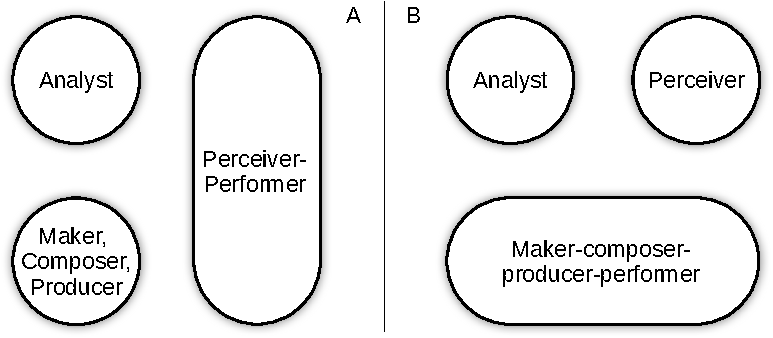
\includegraphics[width=\columnwidth]{figures/44-automatic-quadrant-crop.pdf}
      \caption{Automatic instruments challenge our thinking about traditional musical roles. The users of such instruments can be thought of as perceiver--performers (A) while the creators are a kind of `maker--composer--producer--performer' (B).}
            \label{fig:automatic-quadrant}
}
\end{figure}


\subsection{Conceptual instruments}\label{sec:imaginary}

The final step in the continuum of action--sound separation in acoustic instruments may be somewhat puzzling. It is not about physical instruments at all, but about \emph{conceptual} instruments. One such example is that of \emph{imaginary} instruments. These do not exist in reality, only in our minds. Yet from a philosophical perspective, it makes sense to include also such instruments in this discussion. After all, everyone can imagine that they `listen' to an imaginary instrument. For example, think about a 10-meter long guitar with silver strings. Can you imagine how it sounds? Can you play a tune on it? Can you feel how it would be to touch the strings? While people's imagery of such an imaginary instrument would certainly differ, I believe that thinking about such instruments is also an embodied experience. The category of conceptual instruments would also include what could be called \emph{impossible} instruments. The bike harmonium proposed by \citet{carelman_catalogue_1969} is one such example. It exists in drawings, but can not be physically produced.


\section{Some considerations}

As the discussion above has shown, I support an inclusive approach to what should be considered a musical instrument. However, there are several holes in my theory. Let us consider some of them.


\subsection{Orchestra as an instrument}\label{sec:orchestra}

Can an orchestra be considered an instrument? I would say no, but before we completely abandon the idea, let us evaluate some variations of the question. By definition, an orchestra is composed of several instruments and several musicians. If there is only one musician with multiple instruments, this would usually not be called an orchestra. A borderline case would be a `one-man-band,' in which one person plays on numerous instruments. I would still argue that this is not an orchestra, since it is perceived as one person playing on \emph{multiple} instruments. This also proves my argument that we perceive each of the instruments independently of each other.

Another case is that of a multi-user instrument, where you have one instrument with several performers. As argued above, I think that an acoustic church organ should be considered a multi-user instrument if one person pumps the air while another is playing on the keys. A more generally accepted example is probably a duo playing with four hands on the same piano. Then there are two people playing on the keys of the same instrument.

A more challenging question is whether a group of separate instruments, played by multiple musicians, could somehow be considered \emph{one} instrument. This may seem absurd or irrelevant, but it is a good test case of my theory. The exact number of people and instruments does not matter for this argument, but for a common reference, let us think of a traditional symphony orchestra with a conductor. Suppose you listen to a symphonic concert on headphones, focusing on the sound of the music. In that case, there are good arguments for thinking about the orchestra as a combined sound-producing entity, thus one instrument. For this to work, however, the orchestra would have to work hard to blend. At best, this works effectively, but at worst, it falls apart, and the instruments are heard separately. It also depends on the music being played. Although several 20th-century composers explored different spectral composition techniques, much orchestral music has been composed with a focus on exploring the interplay between various instruments (timbres) and instrument groups (textures). So even from a perceiver's point of view, I would argue that it is common to listen to the orchestra as a combination of individual instruments. This is particularly the case when watching the performance of an orchestra. Seeing the musicians play will make it very difficult to avoid separating the different auditory streams.

I doubt that many orchestra musicians think of the orchestra as one instrument. They have a close physical connection to their own instruments and continuously listen and engage with the others. On the other hand, a composer may think about the orchestra as a `vehicle for sonic expression.' After all, the combination of different timbral qualities defines the orchestra's final sounding result. Orchestration is based on learning how to blend different instrumental timbres and build convergent or divergent sonic textures. Does that make the orchestra into one instrument for the composer? I would say no, based on the spatial and temporal disconnection between the activities of the composer and the orchestra. The composer typically works out-of-time related to the performance situation and is usually not involved in the performance. The composer will also have think about the individual instruments when writing out the individual score parts.

The conductor is the last role we should consider when discussing the orchestra as an instrument. It is perhaps also the most interesting person in this context. One could say that the conductor `plays' the orchestra, at least in the meaning of controlling the final sonic output. This may, in fact, not be so far from the role of a pianolist for a pianola. Someone/something else is producing the musical output, but the conductor/pianolist brings the music `to life.' At least, we may argue for an apparent temporal connection between the conductor and the orchestra. However, the conductor has a disembodied role when it comes to sound production. Even though the conductor controls the orchestra musicians, it is the musicians that produce the sound on their instruments.

All in all, I would argue that it is difficult to say that the orchestra is an instrument. However, it could be considered a `meta-instrument.' It also makes sense to think of both the composer and the conductor as `meta-performers.' They are indirectly involved in music production, with different levels of spatiotemporal distance. As such, their roles may be seen as similar to music producers and engineers. This is something we will get back to when looking at electro-acoustic musicking in the next chapter.


\subsection{The environment as an instrument}\label{sec:space}

As discussed previously, and as summarized in Figure~\ref{fig:excitation-resonance}, the environment is also an essential element in the mental imagery of (musical) sounds.
Humans are generally very capable of separating a sound source from the environment in which it is played. That is also why we can hear a violin playing in anything from a small room to a large cathedral. It has been argued that this is easier to do when the environment has natural characteristics. \citet{traer_perception_2016} conducted a study where they recorded the impulse responses of several hundred rooms, after which they altered the frequency responses slightly. They found that people were better at discriminating sound sources from rooms when the reverberation had natural characteristics. One explanation for this may be an internalization of environmental acoustics through development or evolution.

The sonic properties of a room (the `acoustics'), has in many cases a significant impact on the resultant sound. Both musicians and audiences know to appreciate a good-sounding venue. As \citet[p.307]{howard_acoustics_2007} phrase it:

\begin{quotation}
Reverberation time is an important aspect of sound behavior in a room. If the sound dies away very quickly we perceive the room as being `dead' and we find that listening to, or producing, music within such a space unrewarding. On the other hand when the sound dies away very slowly we perceive the room as being `live.' A live room is preferred to a dead room when it comes to listening to, or producing, live music.
\end{quotation}

Some rooms are built with particular acoustical features. The room acoustics of churches, for example, are of critical importance for the music being performed. Plainchant sounds utterly different inside and outside of reverberant spaces. This is also an example of how music is made for particular environments. For example, churches were a testbed for the development of poly-choral singing, \emph{cori spezzati}, exploring the spatial distribution of sound \citep{schiltz_cori_2018}. However, not many people would argue that a church is an instrument, although it is an exciting line of thought.

Several musical instruments have been designed for particular purposes and venues. The development of louder instruments in the 19th century, for example, was driven by new and larger concert halls \citep{denora_beethoven_1995}. One could also argue that the concert halls could be enlarged because of new and louder musical instruments. Still, most instruments are constructed independently of the performance venue. From a perceptual point of view, I would argue that even though space is essential for shaping the sound of many instruments, it is difficult to say that a room is part of our notion of the instrument. A notable exception is church organs that are custom-built for a particular venue. Here the room could be argued to be the main resonator of the instrument.

The Philips pavilion at the Expo '58 in Brussels is a famous example of the merging of architecture, composition, and instrument design. Here, Iannis Xenakis and Le Corbusier carefully designed a space together with the composed music. As such, one can consider the building itself as a carefully crafted part of a large and complex instrument. The music was played through loudspeakers, though, so this would at best be an example of a hybrid instrument. There are also examples of natural and created sound sculptures  based on acoustic sound-making. We have a beautiful sound sculpture located at the West entrance of the Nationaltheatret train station in Oslo (Figure~\ref{fig:nationaltheatret}). Here people passing by will experience a spectacular flutter echo, which invites for sonic exploration. I always pass by whenever I am around that part of the city. It is fascinating to see how both young and old make sounds and listen to the strange echo before smiling and hurrying down to their train. Such sound sculptures are fascinating, but are they instruments? Some could be, as they may contain both excitatory and modulatory parts. Then they could just be seen as vast acoustic instruments. Others, like the sound sculpture in Oslo, are primarily sound-modifying. The sound-production is done by people passing by. On the other hand, one may argue that exciting a string that resonates in a guitar body is no different from exciting air molecules that resonate in space. So we talk about borderline cases of how far we want to stretch the notion of an instrument.

\begin{figure}[tp]
      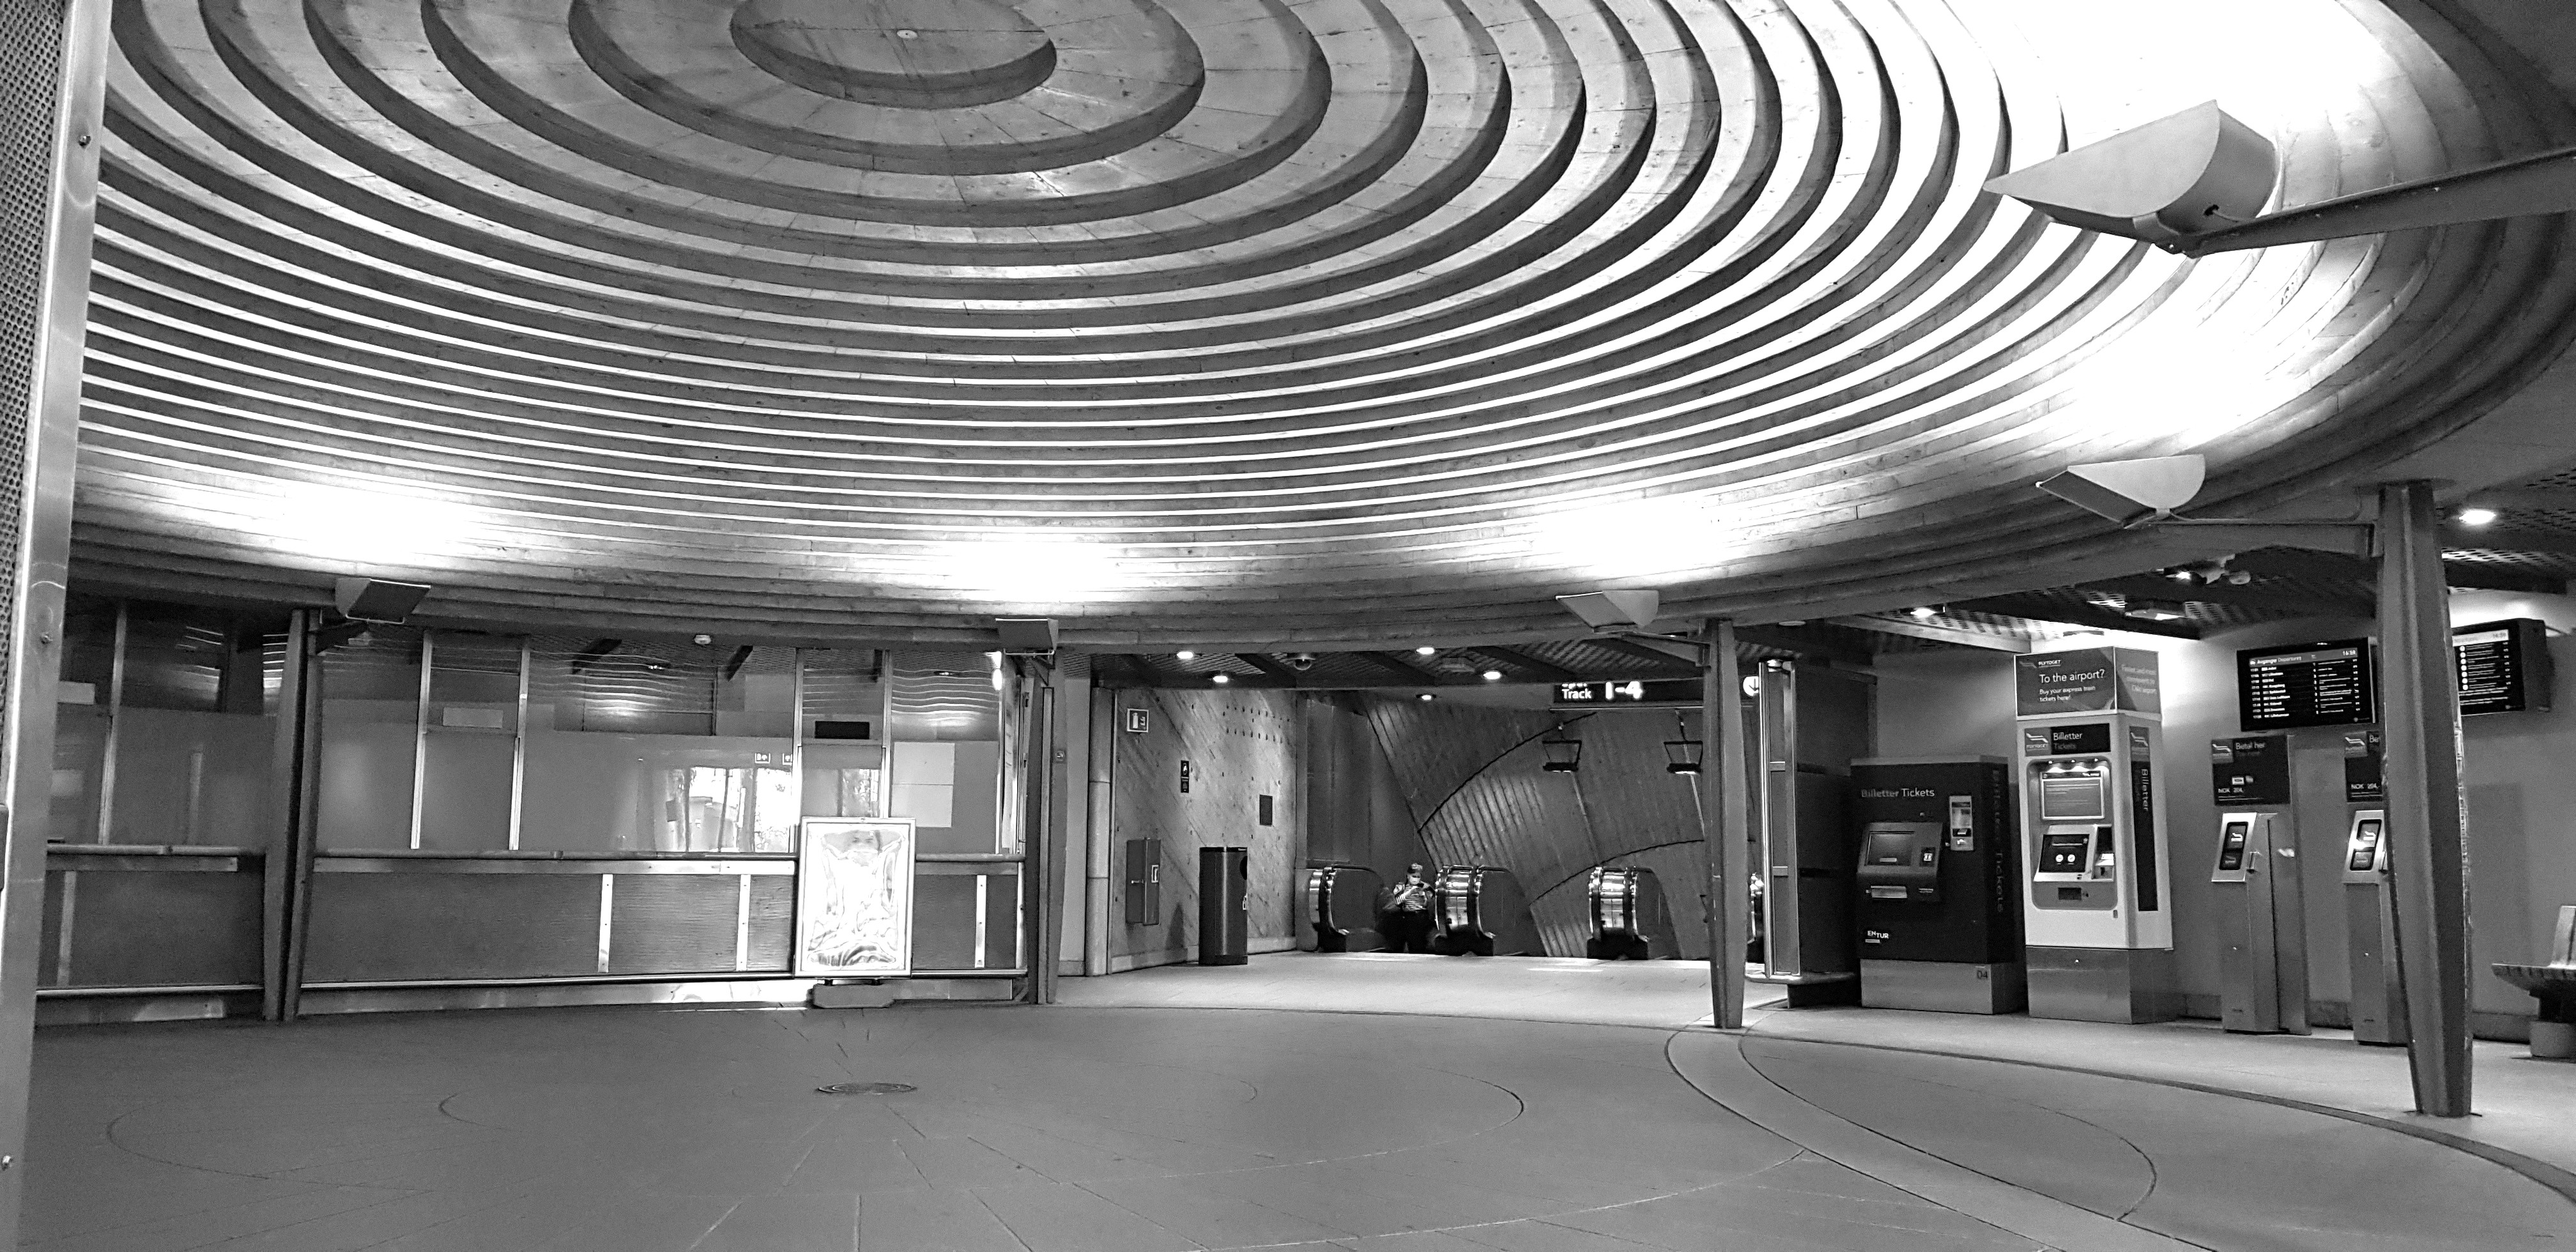
\includegraphics[width=\columnwidth]{figures/45-nationaltheatret.jpg}
      \caption{The West entrance of the Nationaltheatret train station in Oslo is constructed as a sound sculpture featuring a spectacular flutter echo.}
            \label{fig:nationaltheatret}
\end{figure}


\subsection{From sound-maker to music-maker}

An emerging topic is whether music-makers should be considered instruments. I would say yes, but many people refuse my arguments. Some seem to think that instruments are sound-makers that should be hard to play. The argument goes something like this: everyone can play a music box; hence it cannot be an instrument. But why not? What is wrong with anyone being able to play an instrument?

Music boxes are examples of instruments in which a complete musical piece is embedded in the instrument. It is possible to change between different tunes in some music boxes, but they can still only play what is pre-registered in the `score.' This is what \citet{rowe_interactive_1993} would call a `score-driven' system. The performer can control the loudness and tempo, but not much else. Automatic instruments are music-makers that result from the gradual mechanization of musical instruments throughout the centuries. While one may think of such automatic instruments as entirely different from other acoustic instruments, I see more of a continuum. For example, a self-playing piano is a pianola with a system for energy preservation. The pianola is a piano with a system added for recording and playing musical scores. A piano is a harp with an added keyboard mechanism. And a harp is a development of basic string instruments made from a stick and string.

All instruments reflect the (musical) culture they were developed within. Or, in the words of \citet{magnusson_ergomimesis_2018}: `Instruments are impregnated with knowledge expressed as music theory [\ldots] they explain the world.' The piano's keyboard layout has successfully established the twelve-tone equal temperament system as a core part of much of Western music. This is because of the piano's capabilities but perhaps also its lack of ability to explore other tunings and microtonal explorations. Fretless string instruments, on the other hand, afford much richer tonal explorations. Still, one may argue that the construction of string instruments with 4--6 strings and some common tuning standards also influences the music. It is, of course, possible to tune the violin differently, but, as \citet{de_souza_music_2017} argues, some internal musical logic is inevitably built into the construction of the instrument itself.

The gradual `musicification' of instruments from sound-makers to music-makers is also the story of an increasing separation between action and sound. Consider the difference between whistling and playing the silver flute. The first flutes allowed richer and louder sounds than what you could do solely with the mouth. Making holes in the flute allowed for playing discrete pitches. Adding keys to cover the holes ensured more precise playing of those pitches. More mechanical parts made it possible to expand the register. Most instruments have developed over the centuries to allow for more accurate control of intervals, specific timbres, and simultaneous tones \citep{keislar_historical_2009}.

We can also talk about a gradual `verticalization' of musical content as instruments have moved from sound-makers to music-makers. Most instruments with a low action--sound separation are based on playing melodies or rhythmic structures, what we could call `horizontal' musical elements. String-based instruments, such as pianos and guitars, make it possible to develop harmonic structures through chords. Some organs allow for playing additional tones through doublings, and in accordions, you can play complete chords with one finger. All such inventions have given musicians the ability to produce more `vertical' musical complexity in the form of more and more complex tones. All these developments continue in the world of electro-acoustic musicking, which is the topic of the next chapter.
